\chapter{Phonetic Convergence}
\label{chap:phonetic_convergence}

\lettrine{I}{n} this chapter, the concept of accommodation is introduced.
Types of linguistic changes and they way similar terms are used in this work are explained as well.
Finally, a survey of works on phonetic convergence in \acl{hci} lays the ground to the novel work presented in this work.

\pagebreak

\section{Communication accommodation theory}
\label{sec:communication_accommodation_theory}

\todo[inline]{among other things, a survey of language and non-language aspects that were found to converge}
\citet{Racz2020morphological}  % example for accommodation in morphology
\citet{Aubanel2020speaking}  % example for f0

%\subsection{Audience design}
%\label{subsec:audience_design}
%\todo{some start \url{https://en.wikipedia.org/wiki/Audience_design}}

\subsection{Measuring accommodation}
\label{subsec:measuring_accommodation}

\subsection{Limitations of \acl{did} measures}
\label{subsec:limitations_of_did}

\todo[inline]{consider changing the title of this subsec to something more general like "limitations and aspects" (also to be able to write more general things}

\todo[inline]{a few sentences (where?) that *two* aspects are missed by DiD -- temporal and directionality}

%\subsection{Conversation-level accommodation behavior}
%\label{subsec:conversation-level_accommodation_behavior}

Conversations are complex processes that require some expertise and some quantitative analysis to detect and isolate specific patterns in them.
All the more so, since effects may have long, non-linear relations.
A behavior is a complex collection of conducts of a person (and any organism, system, or artificial entity), particularly those towards a certain environment.
The realization of one's behavior over the course of a conversation can communicate information regarding one's state and goals, especially with this deviates from the individual's expected behavior.
The behavior leads to reactions to environmental input and can be modified due to reinforcements from the environment or self-directed motives.
These modifications can occur over time quickly or slowly, consciously or unconsciously, and to greater or lesser extends, which makes them dynamic and thus cannot be defined discretely.
All the above is true also for vocal behaviors, which are expressed in spoken interactions.
Specifically, vocal accommodation reflects dynamic changes during conversation that can be affected by the external speech input of other interlocutors.
It can therefore be beneficial to \textbf{move away from value comparisons in favor of behavior descriptors} to depict an interaction.
This is done by analyzing spoken interactions as entire events with a continuous temporal dimensions as opposed to a comparison between some discrete points in time.
Examining the whole conversation can help, for example, to determine who was leading the changes or when more accommodation occurred.
In this work, such analyses were utilized in \cref{chap:conv_analysis} to determine the leading speaker in each conversation and in \cref{chap:speech_variations_in_hhci} to expose the ongoing changes in the human speaker's productions.

The way speakers accommodate to each other is very unlikely to be linear from beginning to end and can change throughout the conversation.
Therefore, comparing the differences between two discrete, distant points in time might miss or oversimplify some dynamics that occurred between them.
Moreover, comparisons like that must inherently take the view of one speaker instead of looking at the conversation as a complete entity.
Quantitative analyses often leave accommodation hidden or overly-simplified if analyzing a conversation on turn-by-turn basis or by splitting it arbitrarily into two or more parts (often equally-long, non-overlapping time intervals) and directly comparing them using raw values as in \citet{Heldner2010pitch, Rahimi2018weighting, Ibrahim2019fundamental}.
\citet[][p.~15]{DeLooze2014investigating} points out that in these cases it is assumed that accommodation is a strictly local phenomenon where a speaker's utterances is linked exclusively to the other interlocutor's immediate preceding utterance.
Such analyses result in a linear, static representation of the conversation's evolution, from which generalized conclusion are hard to draw.
They might even be inaccurate or misleading, especially when both speakers change their output over time, as demonstrated by \citet{CohenPriva2019limitations}.
That work specifically refer to \ac{did} measurements, where pairs of two discrete points in time are compared to measure accommodation between speakers using the following distance formula\footnote{Note that this way of measuring \ac{did} is commutative and therefore doesn't measure the changes from the view of a specific speaker \citep[unlike,~e.g.,][p.~3]{CohenPriva2019limitations}.}
%
\begin{equation}
	\label{eq:did}
	DiD_{\vec{i},\vec{s}} \coloneqq \sqrt{(\vec{i}_{t + 1}^n - \vec{s}_{t + 1}^n)^2 + (\vec{i}_t^n - \vec{s}_t^n)^2} \equiv \lVert \vec{i} - \vec{s} \rVert_n.
\end{equation}
\eqname{\Acl{did} measure (simplified)}
\noindent
%
\cref{fig:accommodation_types} shows the interaction between two speakers' productions in a hypothetical conversation.
By merely looking at the plot, it is clear that the two speakers do not sustain the same behavior throughout the conversation.
For example, between marks A and B the orange speaker's values go remarkably downwards (though not linearly), while the green speaker remains roughly stable -- i.e., \emph{divergence} (although this can also be seen as an independent changes).
Subsequently, between B and C the distance is generally maintained.
Between C and D \emph{convergence} occurs \textbf{in both speakers}.
Lastly, lagged \emph{synchrony} can be observed between marks D and E.
If compared directly, the lagging might make the value changes look somewhat random.
However, looking at the entire segment, it's clear that the change is similar and is lead by the green speaker.
None of these mutual behavior can be captured by a \ac{did}-based approach.
For instance, comparing the beginning (mark A) and end (mark E) of the conversation would lead to the conclusion that there was no change in the values (illustrated by the corresponding dashed lines).
Similarly, splitting the conversation in two equal halves (A to D and D to E) would make it look like the changes were symmetrical, missing the obviously different behaviors of the speakers in these two halves.
Additionally, the directionality of the convergence between marks C and D will be missed by simple \ac{did} distance measures, which might give the impression that the changed rooted from only one of the speakers.
This could be satisfactory when it can be assumed that such changes can only occur in one speaker, like when talking with some computer-based interlocutor like a \ac{pa} (\cref{sec:convergence_to_natural_and_synthetic_stimuli,sec:vacc}, but not when both speakers' productions may be flexible, like in \ac{hhi} (\cref{sec:analysis_hhi}) or ultimately adaptive \acl{sds} (\cref{sec:adaptive_spoken_dialogue_systems}).
This limitation can be compensated to some extent by examining the \emph{relative} occurring changes \emph{gradually} (\cref{fig:condition_convergence_comparison,subsec:temporal_analysis}).

%Methods used in time series analysis are utilized in this paper to detect and model long-term relations within a conversation.
%This approach offers different types of analyses and emphasizes the temporal aspect of spoken interactions.
%The first is \ac{crqa}, which is proportionate to the conversation's length.
%It measures the \emph{mutual} similarity changes of the speakers throughout the entire conversation in term of recurrence.
%Additionally, it tells when the recurrence segments sustained for longer periods and which speaker lead them.
%\cref{sec:capturing_patterns_in_time_series} explains how this method is used to differentiate the dataset introduced in \cref{sec:dataset_and_feature_extraction} to define different profiles.
%Another method is neural autoencoder (\cref{subsec:dim_reduction}), which can learn non-linear representations in a latent space.
%This technique is good for creating generalized models based on many conversations and speakers.
%By using \ac{vae}, these models become generative and can therefore be used for producing varying speech output of a system fitting to its chosen profile or combination of profiles.
%Finally, \acp{gp} add stochastic Gaussian variability to the yielded output based on the function distribution derived from the models.
%Variations of the base behavior are produced that way.
%This is demonstrated in \cref{subsec:generation_gp_kriging}.

%As discussed in \cref{subsec:conversation-level_accommodation_behavior}, \ac{did} and sequential methods for measuring vocal changes (e.g., accommodation) rely on the chronological, turn-by-turn order of the interaction and their scope is limited to detect local phenomena only.
%Non-linear methods, contrarily, are not dependent on the chronological order of the interaction's turn and can therefore find long-term, more distant relations between the speakers with respect to the target feature.
%For instance, that an accommodation process (or generally closer values) occurred at some point in the beginning and continued at a later time, or that there was a periodic pattern of convergence and divergence throughout the interaction.
%Such phenomena point to more general, conversation-level properties that do not rely on the unfolding chronological order of the turns.
%This is especially useful for long interaction, where various patterns occur a more general view may be insightful (see example in \cref{fig:accommodation_types}).
%
%We take here a different view on the structure of the conversation, namely referring to it as a set of \emph{time series}.
%Time series is a sequence of chronologically ordered values sampled from some data stream along equal time intervals.
%Due to the way the dataset presented in \cref{sec:dataset_and_feature_extraction} is analyzed, the extracted features can be treated as couples of \emph{time series}, one for each speaker in each conversation.
%\todo{examples of where speech is treated as TS (ASR?)}
%Because of the nature of these features (and perhaps any spontaneous, interactive linguistic feature), the resulted time series can be assumed to be non-seasonal and non-stationary.
%\todo{might want to remove this sentence to not commit to this type of data}
%This view on the data enables a new assortment of analysis methods, from which \acf{crqa} and \acf{gp} are demonstrated here (\cref{subsec:crqa,subsec:generation_gp_kriging}).
%
%This recognition as time series opens new methodological possibilities for examining the evolution of these features and their realizations by different speakers in an interaction over time.
%Such methods include, among others, autocorrelation for examining serial dependency and forecasting for transferring information about the time series across time.
%Non-linear analysis methods for time series include, for example, noise reduction and non-linear prediction.
%We utilize here another method that uses phase-space embedding, which describes temporal evolution of trajectories of a dynamic system by projecting their embedding onto some common space.


\begin{figure}[t]
	\centering
	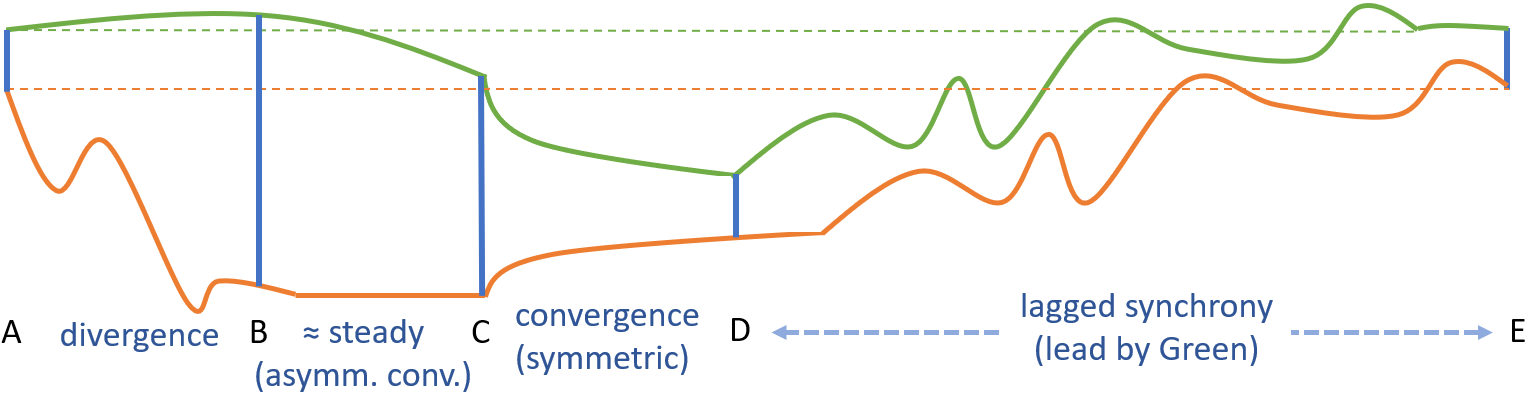
\includegraphics[width=\linewidth]{accommodation_types}
	\caption[Different accommodation types in a conversation]
		{The evolution of a feature's values produced by two speakers represented by the green and orange solid lines.
		The dashed lines connect the corresponding initial and final values of each speaker.
		The letters A to E mark timestamps with behavioral changes.
		Each caption describes the behavior between the two corresponding marks.}
	\label{fig:accommodation_types}
\end{figure}

\section{Pronunciation varieties}
\label{sec:pronunciation_varieties}

\todo[inline]{some introduction...}

\subsection{Variation types}
\label{subsec:variation_types}

The term \enquote{convergence} is a key concept in this work.
To avoid confusion or ambiguous meaning from its use in other fields (like \ac{ml}), its relevant definition will be explained here, along with some other, related terms.
The verb \textit{to converge} is defined by Cambridge Dictionary\footnote{\url{http://dictionary.cambridge.org/dictionary/english/converge}} as moving toward, or merging into, the same point (e.g., roads).
A more non-materialistic definition is given as well: \enquote{If ideas and opinions converge, they gradually become similar}.
Another, somewhat more general, definition to the noun \textit{convergence} is given by Merriam-Webster dictionary\footnote{https://www.merriam-webster.com/dictionary/convergence}: \enquote{the act of converging and especially moving toward union or uniformity}.
As all these definitions suggest, the key idea of this concept is two (or more) entities that \textbf{both} change toward some point and ultimately meet.
In some time-dependent cases, like spoken interactions, there might not be enough time for the entities (the speakers) to meet.
In the scope of phonetic convergence, this still counts as convergence, based on the definition proposed by \citet{Pardo2006phonetic}: \enquote{[\ldots] increase in segmental and suprasegmental similarities between two speakers}.
This also resembles the definition suggested by \citet{Xia2014prosodic}: \enquote{[\ldots] behaviors become more similar over time} (where \enquote{behaviors} refers to different modalities of communications in conversation, e.g., facial expressions, gestures, lexical choices, etc.)

Other terms are sometimes used to describe similar processes, and it is important to make the distinction between those and convergence.
Note that some of the terms are used interchangeably or as synonyms or as hyper-~and~hyponyms in other works, and the distinctions made here, although pretend to unequivocally distinguish between them all, are designated for the scope of this work only.
\todo{find references for each of those}
\todo{create/find figures that describe (at least for some)}
\todo{maybe create a table to compare all of them based on: mutual/one-sided, account for both increase and decrease, has a specific variation as a goal, etc.}
\begin{description}
	\item[accommodation] a general term, comes from accommodation theory (?).
	Refers to both increase and decrease in similarity.
	
	\item[assimilation] implies a one-sided process, where one side changes in a certain way to match the other.
	It is seen more as a process that occurs as a result of a specific area/context.
	This term is typically used in Phonology to describe changes in pronunciation, e.g., when voiceness of a sound changes to match this of the sound adjacent to it.
	For more details and examples, see \cite[][chapter 3.3, pp. 89-98]{Hall2011phonologie}.
	Note that assimilation is only one of the phonological processes (others would be dissimilation, epenthesis, elision, and more), but since it's the once describing two things becoming more similar to each other, it is the one that might be used in this context.
	
	\item[entrainment] \citet{Brennan1996lexical} presents this terms as the (potentially unaware) decision of an interlocutor to start using the same terms as the other interlocutor. This means that one of the interlocutors established the use of the aforementioned term in the interaction.
	The change typically described as categorical (see also \textit{priming} below), which is a key difference from the definition of convergence here.
	This is especially relevant in \ac{hci}, as it is much easier for a computer, due to the vocabulary problem \citep{Furnas1987vocabulary}, to establish such uses.
	\citet{Lopes2013automated} also sees entrainment as something imposed by one side of the interaction, but this time the computer follows the lexical choices of the user.
	This term is sometimes also used a static measure of changes in an interaction. In this context, convergence is usually refereed to the parallel dynamic measure. The difference being comparing changes over the whole interaction or comparing changes in different temporal points in the interaction (For example, between two halves of a session, as done by \citet{Xia2014prosodic}).
	
	\item[priming] is similar to entrainment, but usually works on a larger scope -- both in terms of change and time.
	As oppose to entrainment, e.g., on the lexical level, priming can influence not just the use of one specific term, but a whole semantic field, and more in psycholinguistics contexts.
	For example, it was shown in experiments \cite[e.g.,][]{Meyer1971facilitation, Schvaneveldt1973retrieval} that people will response faster to words from a specific semantic field after being exposed to other words from it (i.e., different words that are semantically related).
	In more general terms, priming changes the likelihood of a person to use specific behavior, typically on some semantic or syntactic level.
	The temporal scope is different as well.
	Priming can have an effect in a longer term than a single interaction, ranging from multiple interactions, hours, days, and up to years.
	This is why priming is often referred to when talking about children \cite[see e.g.\ ][]{Huttenlocher2004syntactic, Wansink2012would}.
	Like entrainment, priming also typically describe categorical change, as oppose to gradual change on a scale (see \textit{entrainment} above and cf.\ \citet{Reitter2006computational} and \citet{Pace2013concept}).
	
	\item[adaptation] usually refers to the capability on the machine side (really only machine side?).
	also refers to a change that will last after the current conversation, e.g., like a user adaptation in \ac{tts}.
	
	\item[alignment] maybe like coordination? Maybe refers more to the time-aspect, that the interlocutors change in the same times, but not necessarily in the same way? Iona talk a bit about alignment in the introduction of the 2018 journal paper. specifically Interactive Alignment Model \citep{Pickering2004behavioral}
	
	\item[synchrony] measures how similar the values of the changes over time.
	However, the changes might be\ldots, i.e., the distance between the speakers does not reduce, but they move in synchrony in terms of absolute values.
	One of the interlocutors will be the ``leader'' of this process, after whom the synchronized changes will be triggered.
	Typically measured using Pearson's correlation coefficient (e.g., as in \citet{Edlund2009pause, Xia2014prosodic}).
	\todo[inline]{\citet{Levitan2011measuring} has a nice visual description for it.}
	
	\item[mimicry] difference from imitation from \url{https://www.voices.com/blog/mimicry_vs_imitation/} use here the \citet{Chartrand1999chameleon} and \citet{Gueguen2009mimicry} and maybe \citet{Parrill2006seeing} reference, mention \textit{Chameleon effect}\ldots
	
	\item[imitation] (also refer to mimicry, as they are similar)similar to mimickry, but is done awarely, where the speaker's goal is to appear as similar as possible to the imitated interlocutor.
	
	\item[mirroring] potentially an aware act. the changes themselves are not planned, but rather automatic to match the target as closely as possible, without considering the output (like an actual mirror).
	
	\item[chameleon effect] \citep{Chartrand1999chameleon}
	
	\item[proximity] indicates how close are the interlocutors to each other as a starting point with respect to their normal behavior.
	For example, their normal f0 compared to their f0 at the beginning of a specific conversation between these two interlocutors.
	This measurement refers only to the beginning of the interaction and serves as a reference point for a specific interaction.
	\todo[inline]{\citet{Levitan2011measuring} has a nice visual description for it.}
	
	\item[coordination] implies cooperation between the interlocutors, i.e. that there is a common goal to achieve.
	Increase or decrease of communication features is in this case a side of effect of this coordination.
	This provides another point of view on the process, namely not to examine the speakers' collaboration based on common changes, but looking at the changes knowing they are collaborating.
	
	\item[inter-speaker influence] a general term to describe a change by a human interlocutor caused by another.
	
	\item[convergence] \ldots
\end{description}

\subsection[Long-term sound change]{Sound change as part of a long-term language evolve process}
\label{subsec:sound_change}

\citet{Ohala1989sound}\\
\citet{Ohala1990phonetics}\\
\citet{Ohala1993phonetics}\\ % this is the main thing
\review{would be cool to have some really old references here. probably there is something in one of Ohala's papers}

\todo[inline]{here talk (very) long term changes (i.e. not in a single conversation). papers of Ohala (especially 1993 book) are good here, and look for more references from there}

\subsection[Short-term phonetic change]{Phonetic change as a short-term social process}
\label{subsec:phonetic_change}

\todo[inline]{start with Harrington's paper about the changes in the queen's phonetics over 60 years or so when talking to the people. explain that this is mid-term change, since it's not a change in language, but also not during a single conversation, but rather over a series of "conversations" with the same crowd}

\section{Phonetic convergence in human-computer interaction}
\label{sec:phonetic_convergence_inh_ci}

introduction\ldots

\citet{Weise2018looking}\\% lexical and prosodic entrainment
\citet{Lewandowski2019phonetic}\\% should be a very good overview paper
\citet{Xiao2015analyzing}\\% speech rate entrainment in HHI
\citet{Cohen2017converging}\\% a bigger work on speech rate tnrainment in HHI
\citet{DeLooze2014investigating}\\% good for when talking about methods

\begin{figure}[t]
	\centering
	\subfigure
	[An illustration of a device's output, which is \emph{not} personalized for each user.
	The same spoken output (in black) is played to all three users.]
	{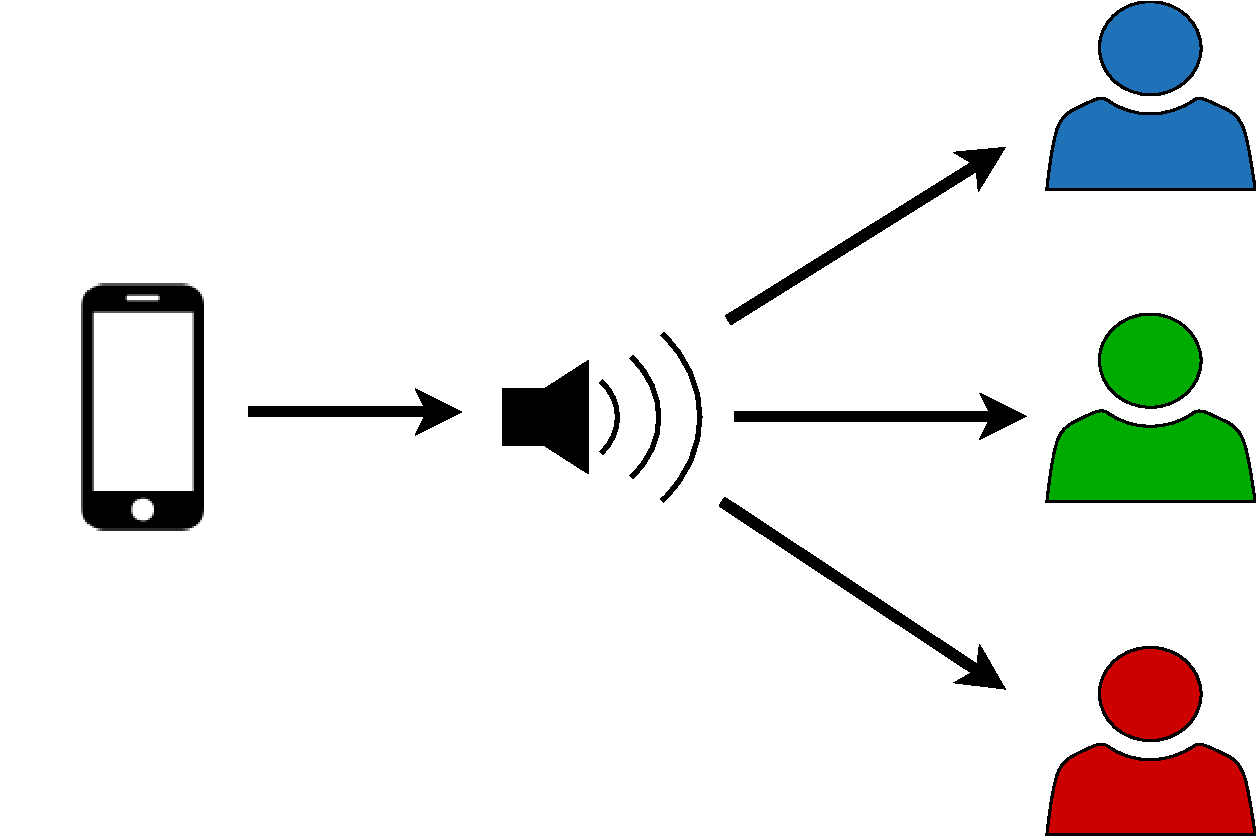
\includegraphics[width=0.45\textwidth]{speech_no_adapt}
		\label{fig:output_not_adapted}} 
	\hfill % no empty line here to avoid staring a new paragraph (figures will be vertically aligned)
	\subfigure
	[An illustration of a device's output, which is \emph{personalized} for each user.
	A different, customized spoken output (in blue, green, and red) is played to each user.]
	{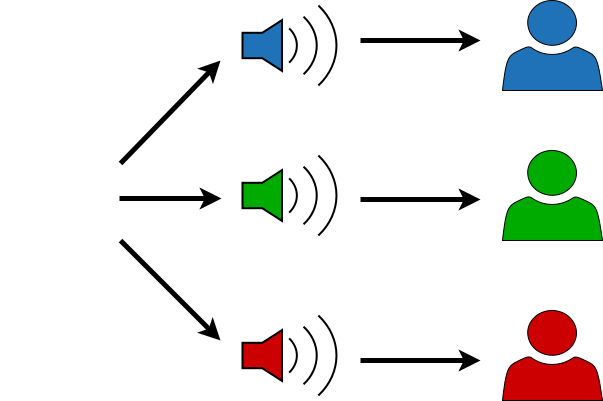
\includegraphics[width=0.45\textwidth]{speech_adapt}
		\label{fig:output_adapted}}
	\caption
	[Static vs.\ adaptive spoken output]
	{Schematic comparison between an interaction with static spoken outputs (on the left) and an interaction with adaptive (i.e., personalized) spoken outputs (on the right).
		The system that adapts to the user makes the interaction tailored to the user's behavior.}
	\label{fig:output_comparison}
\end{figure}

\todo[inline]{taken as-is from SIGdial 2018 subbmitted version. not everyhing belongs here (maybe subsection above?), and the relevant parts should be expanded}

According to \citet{Pardo2006phonetic}, phonetic convergence is defined as an \emph{increase in segmental} \citep[e.g.,][]{Pardo2010conversational, Smith2007prosodic} \emph{and suprasegmental} \citep[e.g.,][]{Walker2015repeat, Shockley2004imitation} \emph{similarity between two interlocutors}.
In contrast to \emph{entrainment}, we use the term \emph{convergence} to describe dynamic, mutual, and non-imposing changes, with potentially non-polarized realizations.
Phonetic convergence has been found in both conversational \citep{Pardo2006phonetic, Lewandowski2012talent} and non-conversational \citep{Babel2014novelty, Shockley2004imitation} scenarios.
There is evidence for phonetic convergence being both an internal mechanism \citep{Pickering2004behavioral} and socially motivated \citep{Kim2011phonetic, Giles1991CAT}.
For instance, convergence \citep{Giles1973mobility} or divergence \citep{Bourhis1977distinctiveness} is triggered with decreasing or increasing social distance between interlocutors, respectively.
Experimental studies on several aspects of phonetic convergence, using a range of methods, have been carried out, e.g., by \citet{Pardo2013measuring, Nielsen2011specificity, Shockley2004imitation}.

Previous studies of phonetic convergence in spontaneous dyadic conversations have focused on speech rate \citep{Schweitzer2016exemplar} and timing-related phenomena \citep{Putman1984conception}, pitch \citep{Gessinger2018pitch, Schweitzer2017visibility}, intensity \citep{Levitan2011measuring, Natale1975convergence}, and perceived attractiveness \citep{Michalsky2017pitch}.
Phonetic convergence is often examined in the scope of shadowing experiments, in which the participants are asked to repeat utterances spoken by an interlocutor \citep{Pardo2017phonetic, Dias2016visibilivty, Walker2015repeat}.
This is typically done with single words as targets.
The experiment showcasing our system in \cref{sec:showcase} uses whole sentences as stimuli, in which the target features are embedded, making it a semi-conversational \ac{hci} setting.

% \input{chapters/introduction/spokendialoguesystems}